\documentclass{beamer}

% Theme choice
\usetheme{Madrid}

% Optional packages
\usepackage{graphicx} % For including images
\usepackage{amsmath}  % For math symbols and formulas
\usepackage{hyperref} % For hyperlinks

\title[Linux]{Linux}
\author{Obolenskiy Arseniy, Nesterov Alexander}
\institute{ITLab}

\date{\today}

% Redefine the footline to display both the short title and the org name
\setbeamertemplate{footline}{
  \leavevmode%
  \hbox{%
    \begin{beamercolorbox}[wd=.45\paperwidth,ht=2.5ex,dp=1ex,leftskip=1em,center]{author in head/foot}%
        \usebeamerfont{author in head/foot}\insertshortinstitute % Displays the university name
    \end{beamercolorbox}%
    \begin{beamercolorbox}[wd=.45\paperwidth,ht=2.5ex,dp=1ex,leftskip=1em,center]{author in head/foot}%
      \usebeamerfont{author in head/foot}\insertshorttitle % Displays the short title
    \end{beamercolorbox}%
    \begin{beamercolorbox}[wd=.1\paperwidth,ht=2.5ex,dp=1ex,rightskip=1em,center]{author in head/foot}%
      \usebeamerfont{author in head/foot}\insertframenumber{} / \inserttotalframenumber
    \end{beamercolorbox}}%
  \vskip0pt%
}

\begin{document}

\begin{frame}
    \titlepage
\end{frame}

\begin{frame}{Contents}
    \tableofcontents
\end{frame}

\section{Introduction}


\begin{frame}{What is Linux?}
  \begin{minipage}[t]{0.6\textwidth}
    Linux is a generic name for a family of open-source Unix-like operating systems based on the Linux kernel. \\
    Linux operating system is widely used in servers, personal computers, embedded systems, and other devices. It is built on the Linux kernel, which is the core of the operating system that manages communication between hardware and software.
    \vspace{10pt}
    \\
    \footnotesize Source: \href{https://en.m.wikipedia.org/wiki/File:Tux.svg}{https://en.m.wikipedia.org/wiki/File:Tux.svg}
  \end{minipage}
  \hfill
  \begin{minipage}[t]{0.35\textwidth}
    \begin{figure}[h]
      
\includegraphics[width=0.7\textwidth]{images/tux.png}
    \end{figure}
  \end{minipage}
\end{frame}

\begin{frame}{Why Linux?}
  \begin{itemize}
    \item Free and open-source operating system
    \item Open-source nature and customization flexibility
    \item Wide range of applications and tools
    \item Enhanced security
    \item High stability and reliability
    \item Community support and resources
    \item Cost-effectiveness compared to proprietary software
    \item Scalability for handling large amounts of data and traffic
    \item Compatibility with modern DevOps practices and configuration management
    \item Support for visualization
  \end{itemize}

  \footnotesize Source: \href{https://www.logicmonitor.com/blog/9-reasons-linux-is-a-popular-choice-for-servers}{https://www.logicmonitor.com/blog/9-reasons-linux-is-a-popular-choice-for-servers}
\end{frame}

\begin{frame}{Where Linux is used?}
  \begin{itemize}
    \item Servers
    \item Supercomputers
    \item Personal computers
    \item Embedded systems
    \item Networking equipment
    \item and many others...
  \end{itemize}
\end{frame}

\section{History}

\begin{frame}{UNIX}
  \begin{itemize}
    \item Developed in AT\&T's Bell Labs in late 60s
    \item Designed as a multiuser, multitasking system
    \item Influenced many subsequent operating systems
  \end{itemize}
\end{frame}


\begin{frame}{UNIX history}
  \begin{itemize}
    \item Origins at Bell Labs (1969-1970)
    \item UNIX Expansion (1970s)
    \begin{itemize}
      \footnotesize
      \item Version 1 (1971): The first official version was released
      \item Academic Adoption: By 1973, UNIX had been rewritten in C, making it more portable
      \item Influence on Academia: UNIX became a popular teaching and research tool in academic circles, and many computer science students learned programming in this environment
    \end{itemize}
    \item Commercialization and Fragmentation (1980s)
    \begin{itemize}
      \footnotesize
      \item Version 1 (1971): AT\&T began to commercialize UNIX more aggressively
      \item System V (1983): AT\&T's commercial version of UNIX, called System V, became a standard for many commercial UNIX systems. However, BSD continued to evolve separately, leading to a fragmentation of UNIX versions
    \end{itemize}
    \item UNIX Wars (1980s-1990s)
    \begin{itemize}
      \footnotesize
      \item Many different versions appeared
      \item POSIX Standard was introduced
    \end{itemize}
    \item Rise of Linux and Open Source (1990s)
    \item Modern UNIX and Legacy (2000s - Present)
  \end{itemize}
\end{frame}

\begin{frame}{UNIX timeline}
  \begin{figure}[h]
    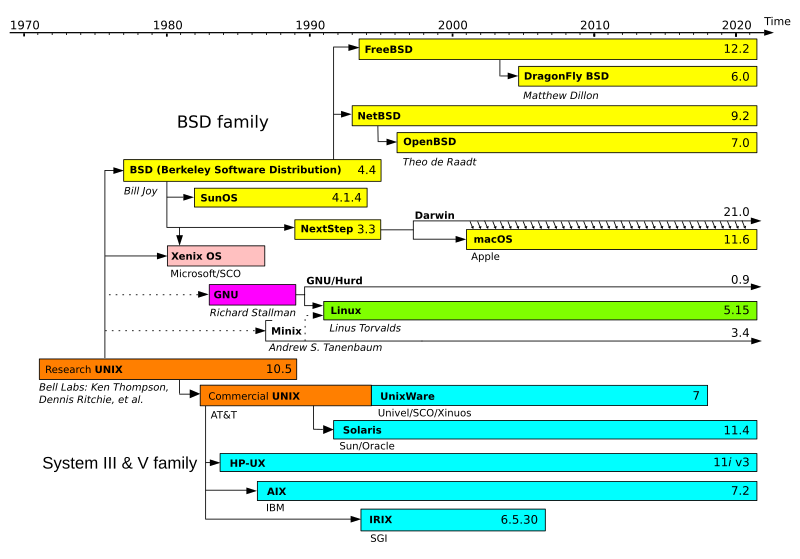
\includegraphics[width=0.85\textwidth]{images/unix-timeline.png}
  \end{figure}

  \footnotesize Source: \href{https://en.m.wikipedia.org/wiki/File:Unix_timeline.en.svg}{https://en.m.wikipedia.org/wiki/File:Unix\_timeline.en.svg}
\end{frame}

\begin{frame}{Linux history}
  \begin{itemize}
    \item Created by Linus Torvalds in 1991
    \item Initially developed as a hobby project inspired by UNIX
    \item Released under the GNU General Public License (GPL)
    \item Although Linux is not technically UNIX, it follows the UNIX philosophy and provides similar functionality
    \item It became popular due to its open-source nature and flexibility
  \end{itemize}
\end{frame}

\begin{frame}{GNU/Linux}
  \begin{minipage}[t]{0.6\textwidth}
    \begin{itemize}
      \item GNU Project initiated by Richard Stallman in 1983
      \item Aimed to create a free Unix-like operating system
      \item Linux kernel combined with GNU tools forms GNU/Linux
    \end{itemize}
  \end{minipage}
  \hfill
  \begin{minipage}[t]{0.35\textwidth}
    \begin{figure}[h]
      
\includegraphics[width=0.7\textwidth]{images/tux.png}
    \end{figure}
  \end{minipage}
\end{frame}

\section{Linux}

\begin{frame}{Linux supported platforms}
  \begin{itemize}
    \item x86 (32-bit)
    \item x86\_64 (64-bit)
    \item ARM (64-bit)
    \item AArch64 (ARM 64-bit)
    \item RISC-V (32-bit and 64-bit)
    \item PowerPC (32-bit and 64-bit)
    \item MIPS (32-bit and 64-bit)
    \item SPARC (32-bit and 64-bit)
    \item Itanium (IA-64)
    \item LoongArch
    \item and many others...
  \end{itemize}

  \footnotesize Full up-to-date list: \href{https://en.wikipedia.org/wiki/List_of_Linux-supported_computer_architectures}{https://en.wikipedia.org/wiki/List\_of\_Linux-supported\_computer\_architectures}
\end{frame}

\begin{frame}{Linux distributions}
  What is a Distribution?

  A Linux distribution is an operating system made from a software collection, which includes the Linux kernel and often a package management system.

  Examples:
  \begin{itemize}
    \item Ubuntu
    \item Fedora
    \item Debian
    \item Arch Linux
    \item Red Hat Enterprise Linux
  \end{itemize}
\end{frame}

\begin{frame}{Debian and Ubuntu}
  \begin{minipage}[t]{0.65\textwidth}
    Debian:
    \begin{itemize}
      \item Debian was first created in 1993 by Ian Murdock
      \item One of the oldest distributions
      \item Known for its stability and robustness
    \end{itemize}
  \end{minipage}
  \hfill
  \begin{minipage}[t]{0.3\textwidth}
    \begin{figure}[h]
      
\includegraphics[width=0.3\textwidth]{images/debian.jpg}
    \end{figure}
  \end{minipage}

  \begin{minipage}[t]{0.65\textwidth}
    Ubuntu:
    \begin{itemize}
      \item Ubuntu was first released on October, 2004. It was developed by Canonical Ltd., founded by Mark Shuttleworth, a South African entrepreneur
      \item Based on Debian
      \item Created user-friendly and widely used for desktops
      \item Has regular releases and strong community support
    \end{itemize}
  \end{minipage}
  \hfill
  \begin{minipage}[t]{0.3\textwidth}
    \begin{figure}[h]
      
\includegraphics[width=0.7\textwidth]{images/ubuntu.png}
    \end{figure}
  \end{minipage}
\end{frame}

\begin{frame}{Package managers}
  \begin{itemize}
    \item \texttt{APT (Advanced Package Tool)} for Debian-based systems.
    \item \texttt{YUM/DNF} for Red Hat-based systems.
    \item \texttt{Pacman} for Arch Linux.
  \end{itemize}
  \begin{block}{Purpose of Package Managers}
    Package managers simplify the process of installing, updating, and removing software packages.
  \end{block}
\end{frame}

\section{Basic Linux commands}

\begin{frame}{File system overview}
  \begin{figure}[h]
    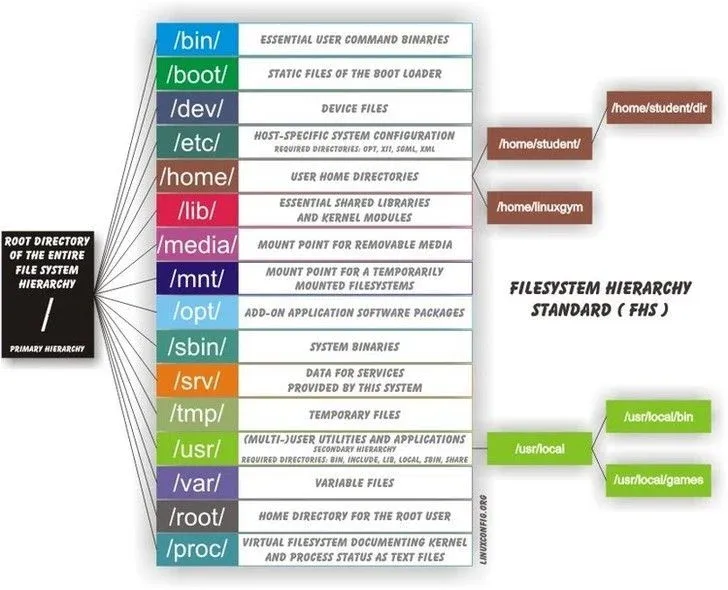
\includegraphics[height=0.81\textheight]{images/linux-fs.png}
  \end{figure}

  \footnotesize Source: \href{https://blog.fourninecloud.com/linux-file-system-hierarchy-explained-1d80b2cee03c}{Linux File System Hierarchy - Explained}
\end{frame}

\begin{frame}{Files navigation}
  \begin{itemize}
    \item \texttt{pwd} : Print working directory
    \item \texttt{ls} : List directory contents
    \item \texttt{cd} : Change directory
    \item \texttt{mkdir} : Create a new directory
  \end{itemize}
  \begin{exampleblock}{Examples}
    \begin{itemize}
      \item \texttt{ls -l} : Detailed list
      \item \texttt{cd /home/user} : Navigate to user's home
    \end{itemize}
  \end{exampleblock}
\end{frame}

\begin{frame}{File Manipulations}
  \begin{itemize}
    \item \texttt{touch} : Create an empty file or update timestamp
    \item \texttt{cp} : Copy files or directories
    \item \texttt{mv} : Move or rename files
    \item \texttt{rm} : Remove files or directories
    \item \texttt{cat} : Concatenate and display files
  \end{itemize}
  \begin{exampleblock}{Examples}
    \begin{itemize}
      \item \texttt{touch file.txt} : Create a new file
      \item \texttt{rm -r folder} : Remove a directory and its contents
    \end{itemize}
  \end{exampleblock}
\end{frame}

\begin{frame}{Text Editors}
  \begin{itemize}
    \item \textbf{nano} : Simple text editor
    \item \textbf{vim} : Advanced text editor with modal editing
    \item \textbf{code} : Visual Studio Code (GUI only)
  \end{itemize}
  \begin{exampleblock}{Opening a File}
    \begin{itemize}
      \item \texttt{nano file.txt}
      \item \texttt{vim file.txt}
      \item \texttt{code file.txt}
    \end{itemize}
  \end{exampleblock}
\end{frame}

\begin{frame}{Linux command line demo}
  Demo
\end{frame}

\begin{frame}
    \centering
    \Huge{Thank You!}
\end{frame}

\begin{frame}{References}
  \begin{enumerate}
    \item The Linux command line for beginners \href{https://ubuntu.com/tutorials/command-line-for-beginners}{https://ubuntu.com/tutorials/command-line-for-beginners}
    \item The Linux command line for beginners \href{https://ubuntu.com/tutorials/command-line-for-beginners}{https://ubuntu.com/tutorials/command-line-for-beginners}
    \item Top 50+ Linux Commands You MUST Know \href{https://www.digitalocean.com/community/tutorials/linux-commands}{https://www.digitalocean.com/community/tutorials/linux-commands}
  \end{enumerate}
\end{frame}

\end{document}
